\section{Case Study B: OpenCL Thread Coarsening Factor}
\label{sec:deeptune-case-study-b}

Thread coarsening is an optimisation for parallel programs in which the operations of two or more threads are fused together. This optimisation can prove beneficial on certain combinations of programs and architectures, for example, programs with a large potential for Instruction-level Parallelism on Very Long Instruction Word architectures.

\subsection{State-of-the-art} \citeauthor{Magni2014} present a predictive model for OpenCL thread coarsening in~\cite{Magni2014}. They implement an iterative heuristic which determines whether a given program would benefit from coarsening. If yes, then the program is coarsened, and the process repeats, allowing further coarsening. In this manner, the problem is reduced from a multi-label classification problem into a series of binary decisions, shown in Figure~\ref{fig:cf-magni}. They select from one of six possible coarsening factors: $(1, 2, 4, 8, 16, 32)$, divided into 5 binary choices.

\begin{figure}
  \centering %
  \subfloat[\citeauthor{Magni2014} cascading binary model.]{%
    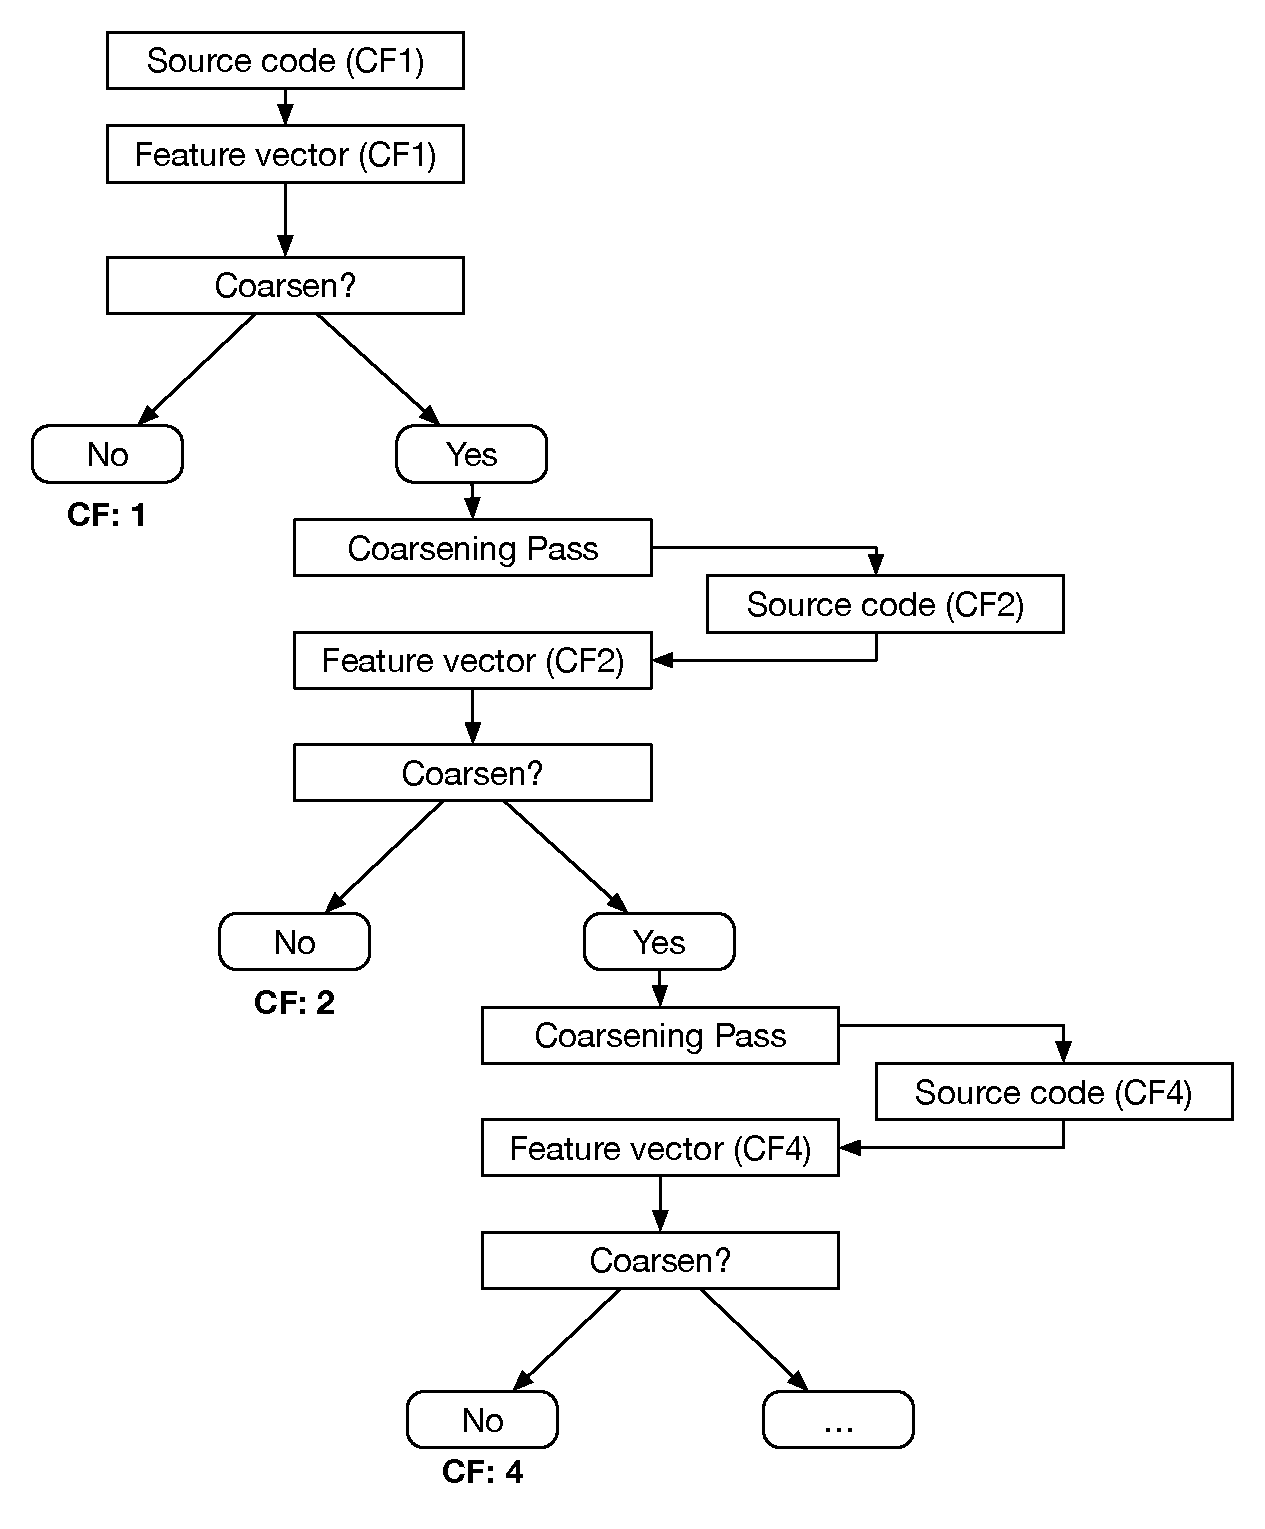
\includegraphics[width=.95\columnwidth]{img/cf-magni}%
    \label{fig:cf-magni}
  }\\*%
  \subfloat[Proposed approach.]{%
      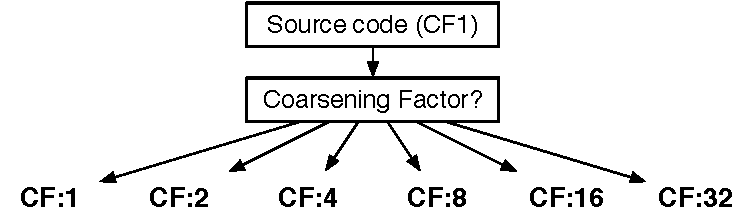
\includegraphics[width=.75\columnwidth]{img/cf-deeptune}%
      \label{fig:cf-deeptune}
  }%
  \caption[Predicting OpenCL thread coarsening factors.]{%
      Two approaches for predicting coarsening factor (CF) of OpenCL kernels.
      \citeauthor{Magni2014} reduce the multi-label classification problem to a
      series of binary decisions, by iteratively applying the optimisation and
      computing new feature vectors. Our approach simply predicts the coarsening
      factor directly from the source code.%
  }
  \label{fig:cascading-nn}
\end{figure}

\begin{table}
  \rowcolors{2}{gray!25}{white}
  \centering%
    \begin{tabular}{| l l |}
      \hline
      \rowcolor{gray!50}
      \textbf{Name} & \textbf{Description} \\
      \hline
      \texttt{BasicBlocks} & \#.\ basic blocks \\
      \texttt{Branches} & \#.\ branches \\
      \texttt{DivInsts} & \#.\ divergent instructions \\
      \texttt{DivRegionInsts} & \#.\ instructions in divergent regions \\
      \texttt{DivRegionInstsRatio} & \#.\ instr. in divergent regions / total instructions \\
      \texttt{DivRegions} & \#.\ divergent regions \\
      \texttt{TotInsts} & \#.\ instructions \\
      \texttt{FPInsts} & \#.\ floating point instructions \\
      \texttt{ILP} & average ILP / basic block \\
      \texttt{Int/FP Inst Ratio} & \#.\ branches \\
      \texttt{IntInsts} & \#.\ integer instructions \\
      \texttt{MathFunctions} & \#.\ match builtin functions \\
      \texttt{MLP} & average MLP / basic block \\
      \texttt{Loads} & \#.\ loads \\
      \texttt{Stores} & \#.\ stores \\
      \texttt{UniformLoads} & \#.\ loads unaffected by coarsening direction \\
      \texttt{Barriers} & \#.\ barriers \\
      \hline
    \end{tabular}%
    \label{tab:features-pact14-raw}%
  \caption[\emph{Magni et al.\ }features for predicting thread coarsening]{%
    Candidate features used by \emph{Magni et al.\ }for predicting thread
    coarsening. From these values, they compute relative deltas for each
    iteration of coarsening, then use PCA for selection.%
  }%
  \label{tab:magni-features} %
\end{table}


\paragraph*{Expert Chosen Features}

\citeauthor{Magni2014} followed a very comprehensive feature engineering process. 17 candidate features were assembled from previous studies of performance counters and computed theoretical values~\cite{Magni2,Sim2012}. For each candidate feature, they compute its coarsening \emph{delta}, reflecting the change in each feature value caused by coarsening: $f_{\Delta} = (f_{after} - f_{before}) / f_{before}$, adding it to the feature set. Then they use Principal Component Analysis (PCA) on the 34 candidates and selected the first 7 principal components, accounting for 95\% of variance in the space.

\subsection{Experimental Setup}

The experimental setup of \citeauthor{Magni2014}~\cite{Magni2014} is replicated for this case study. The thread coarsening optimisation is evaluated on 17 programs, listed in Table~\ref{tab:pact-benchmarks}. Four different GPU architectures are used, listed in Table~\ref{tab:pact-platforms}.

\begin{table}
  \centering %
  \rowcolors{2}{gray!25}{white}
  \begin{tabular}{| l r r r |}
    \hline
    \rowcolor{gray!50}
    & \textbf{Version} & \textbf{\#. benchmarks} & \textbf{\#. kernels}\\
    \hline
    \textbf{NVIDIA SDK} & 4.2 & 3 & 3 \\
    \textbf{AMD SDK} & 3.0 & 10 & 10 \\
    \textbf{Parboil~\cite{Stratton2012}} & 0.2 & 4 & 4 \\
    \textbf{Total} & - & 17 & 17 \\
    \hline
  \end{tabular}
  \caption[Benchmarks used in Case Study B]{%
    Benchmarks used in Case Study B.%
  }
  \label{tab:pact-benchmarks}
\end{table}

\begin{table}[t!]
  \centering %
  \rowcolors{2}{gray!25}{white}
  \begin{tabular}{| l l l l |}
    \hline
    \rowcolor{gray!50}
    & \textbf{Frequency} & \textbf{Memory} & \textbf{Driver} \\
    \hline
    \textbf{AMD HD 5900} & 725 MHz & 2GB & AMD 1124.2 \\
    \textbf{AMD Tahiti 7970} & 1000 MHz & 3GB & AMD 1084.4 \\
    \textbf{NVIDIA GTX 480} & 700 MHz & 1536 MB & NVIDIA 304.54 \\
    \textbf{NVIDIA K20c} & 706 MHz & 5GB & NVIDIA 331.20 \\
    \hline
  \end{tabular}
  \caption[Experimental platforms used in Case Study B]{%
    Experimental platforms used in Case Study B.%
  }
  \label{tab:pact-platforms}
\end{table}


\paragraph*{DeepTune Configuration}

Figure~\ref{fig:nn}b shows the artificial neural network configuration. The OpenCL kernel is the sole input the coarsening factor is the predicted output.

\paragraph*{Model Evaluation}

Compared to Case Study A, the size of the evaluation is small. We use \emph{leave-one-out cross-validation} to evaluate the models. For each program, a model is trained on data from all other programs and used to predict the coarsening factor of the excluded program.

The parameters of the artificial neural network are not described in~\cite{Magni2014}, so an additional, \emph{nested} cross-validation process is used to find the optimal model parameters. For every program in the training set, a grid search of 48 combinations of network parameters is performed. The best performing parameter configuration is selected from these 768 results to train a model for prediction on the excluded program. This nested cross-validation is repeated for each of the training sets. No such tuning of hyper-parameters is performed for DeepTune.


\subsection{Comparison to Case Study A}

For the two different optimisation heuristics, the authors arrived at very different predictive model designs, with very different features. By contrast, the DeepSmith approach is exactly the same for both problems. None of DeepTune's parameters were tuned for the case studies presented above. Their settings represent conservative choices expected to work reasonably well for most scenarios.

Table~\ref{tab:nn-size} shows the similarity of the models. The only difference between the network designs is the auxiliary inputs for Case Study A and the different number of optimisation decisions. The differences between DeepTune configurations is only two lines of code: the first, adding the two auxiliary inputs; the second, increasing the size of the output layer for Case Study B from two neurons to six. The description of these differences is larger than the differences themselves.

\begin{table}
  \centering
  \rowcolors{2}{white}{gray!25}
  \begin{tabular}{| l r r | r r |}
    \hline
    \rowcolor{gray!50}
    & \multicolumn{2}{c}{\textbf{\#.\ neurons}} & \multicolumn{2}{c}{\textbf{\#.\ parameters}} \\
    \rowcolor{gray!50}
    & \textbf{HM} & \textbf{CF} & \textbf{HM} & \textbf{CF} \\
    \hline
    \textbf{Embedding} & 64 & 64 & ,256 & 8,256 \\
    \textbf{LSTM\_1} & 64 & 64 & 33,024 & 33,024 \\
    \textbf{LSTM\_2} & 64 & 64 & 33,024 & 33,024 \\
    \textbf{Concatenate} & 64 + 2 & - & - & - \\
    \textbf{Batch Normalisation} & 66 & 64 & 264 & 256 \\
    \textbf{DNN\_1} & 32 & 32 & 2,144 & 2,080 \\
    \textbf{DNN\_2} & 2 & 6 & 66 & 198 \\
    \hline
    \textbf{Total} & & & 76,778 & 76,838 \\
    \hline
  \end{tabular}
  \caption[DeepTune model parameters]{%
    The size and number of parameters of the DeepTune components of
    Figure~\ref{fig:nn}, configured for heterogeneous mapping (HM) and
    coarsening factor (CF).%
  }
  \label{tab:nn-size}
\end{table}



\subsection{Experimental Results}

Exploiting thread coarsening for OpenCL kernels is a difficult task. On average, coarsening slows programs down. The speedup attainable by a perfect heuristic is only $1.36\times$.

Figures~\ref{fig:pact-speedup-left} and~\ref{fig:pact-speedup-right} show speedups achieved by the \citeauthor{Magni2014} and DeepTune models for all programs and platforms. The performance of programs without coarsening is used as a baseline. On the four experimental platforms (AMD HD 5900, Tahiti 7970, NVIDIA GTX 480, and Tesla K20c), the \citeauthor{Magni2014} model achieves average speedups of $1.21\times$, $1.01\times$, $0.86\times$, and $0.94\times$, respectively. DeepTune outperforms this, achieving speedups of $1.10\times$, $1.05\times$, $1.10\times$, and $0.99\times$.

Some programs --- especially those with large divergent regions or indirect memory accesses --- respond very poorly to coarsening. No performance improvement is possible on the \texttt{mvCoal} and \texttt{spmv} programs. Both models fail to achieve positive average speedups on the NVIDIA Tesla K20c, because thread coarsening does not give performance gains for the majority of the programs on this platform.

The disappointing results for both predictive models may be attributed to the small training program set (only 17 programs in total). As a result, the models suffer from sparse training data. In Chapter~\ref{chap:clgen} of this thesis, a methodology for overcoming data sparsity using additional programs is presented. In this instance, the shared structure of the DeepTune models between the two case studies enables an alternate strategy to overcome data scarcity. The following subsection describes and tests a novel strategy for training optimisation heuristics on a small number of programs by exploiting knowledge learned from other optimisation domains.
